\documentclass{article}
\usepackage[utf8]{inputenc}
\usepackage{longtable}
\usepackage{authblk}
\usepackage{adjustbox}

\usepackage{natbib}


\title{INFORMACION ESTADISTICA DE LA POBLACION DE COLOMBIA}
% autores
%\renewcommand\Authand{, y }
\author[1]{\normalsize Marlon Fabian Titua\~na De La Vega}
\affil[1]{\small  Escuela de Ingeniería,Universidad de los Andes\\
\texttt{{mf.tituanad}@uniandes.edu.co}}


\date{30 de Junio de 2018}



\usepackage{Sweave}
\begin{document}
\Sconcordance{concordance:Proyecto_Final.tex:Proyecto_Final.Rnw:%
1 21 1 1 0 13 1 1 6 1 5 10 1 1 5 14 0 1 2 12 1 1 10 1 4 13 1 1 11 1 3 8 %
1 1 6 12 0 1 3 1 1 1 9 13 0 1 2 6 1 2 2 8 1 1 8 1 1 1 9 31 0 1 2 13 1 1 %
21 1 1 1 34 4 1 1 29 1 3 12 1}

\maketitle
\begin{abstract}
Este  paper trata de un estudio estadistico de la poblacion Son escasos los estudios sobre el desarrollo económico colombiano que abarquen la primera mitad del siglo XX . A excepción de los trabajos sobre la economía del café y el surgimiento del proceso de industrialización durante los años veinte y treinta, casi todas las interpretaciones sobre el desempeño de la economía real parten de 1950. En el caso del sector agropecuario las investigaciones que cubren el
período 1905-1950 son mínimas, no existe información estadística confiable del agregado sectorial como tampoco del subsector agrícola sin café (salvo algunos estudios para productos transables) y ningún estudio sobre la producción ganadera en el ámbito nacional.
Los desarrollos recientes de la historia económica están empeñados en la aplicación de un método científico en esta área de las ciencias sociales/1
, mediante el cual se combine la teoría económica, el uso riguroso de las fuentes primarias para poder cuantificar y la comprobación estricta de las hipótesis. En consecuencia, y de acuerdo con las deficiencias en las series reales de la economía nacional, hemos armado este arsenal de estadísticas cuidadosamente construidas, con el fin de poder utilizar la economía sobre bases más confiables y plantear hipótesis contrastables con mejores métodos de verificación.de lo mi primer trabajo en exploracion y modelamiento de indices usando LATEX. Este trabajo lo he hecho bajo la filosa de trabajo replicable.
\end{abstract}
\section*{Introducción}

Aqui les presento mi investigacion sobre diversos indices sociales  de colombia Colombia entre 1915 y 1950 era una economía que dependía del sector primario y en menor medida de una naciente industria, por tanto, la cuantificación de la producción agropecuaria es vital para encontrar la composición del producto durante esos años. Sin embargo, no existía un responsable de esta labor \cite{macqueen_methods_nodate}. En los primeros años del siglo XX fue la Oficina de Estadística del Ministerio de Hacienda, la encargada de producir algunas cifras estadísticas (en estrecha relación con su utilidad fiscal) y sólo con la reforma institucional de los años veinte esta labor se traslado a la Contraloría General de la Nación, entidad que empezó a publicar los Anuarios Generales de Estadística y los Anuarios de Comercio Exterior \cite{gutierrez_cesar_nodate-1}.  En los años cincuenta se estableció El Departamento Administrativo Nacional de Estadística, organismo que desde entonces tiene la mayor responsabilidad sobre las estadísticas de producción, precios, población e ingresos y gastos, entre otras. Este proyecto se realizara en Latex



Comencemos viendo que hay en la sección \ref{univariada} en la pagina \pageref{univariada}.




\section{Exploracion Univariada}\label{univariada}

La publicación del Atlas Estadístico de Colombia que el DANE presenta al servicio de los colombianos y ciudadanos del mundo interesados en la realidad de nuestro país, tiene como objetivo brindar, a través de la cartografía temática, los textos, la semiología gráfica y las ayudas visuales complementarias, un perfil de las principales configuraciones poblacionales y territoriales de Colombia sobre aspectos demográficos, sociales y económicos. Como apreciamos en la Tabla \ref{stats}.

%Para resaltar lo anterior, tenemos la Figura \ref{barplots} en la pagina \pageref{barplots}. 

% Table created by stargazer v.5.2.2 by Marek Hlavac, Harvard University. E-mail: hlavac at fas.harvard.edu
% Date and time: sáb., jun. 30, 2018 - 3:06:45 p. m.
\begin{table}[!htbp] \centering 
  \caption{Medidas estadisticas} 
  \label{stats} 
\begin{tabular}{@{\extracolsep{5pt}}lcccc} 
\\[-1.8ex]\hline 
\hline \\[-1.8ex] 
Statistic & \multicolumn{1}{c}{N} & \multicolumn{1}{c}{Median} & \multicolumn{1}{c}{Max} & \multicolumn{1}{c}{Min} \\ 
\hline \\[-1.8ex] 
IDH & 32 & 0.804 & 0.879 & 0.691 \\ 
Población.Cabecera & 32 & 717,197 & 10,070,801 & 13,090 \\ 
Población.Resto & 32 & 268,111.5 & 1,428,858 & 21,926 \\ 
\hline \\[-1.8ex] 
\end{tabular} 
\end{table} 
%%%%% figure

El antecedente inmediato de la presente publicación es el libro de Dinámicas Demográficas del Espacio Colombiano elaborado por el DANE en 1999 en estrecha colaboración con el Crece (Centro de Estudios Regionales, Cafeteros y Empresariales) y el IRD (Institut de Recherche pour le Developpement) de Francia, como parte de un proyecto conjunto de los países andinos enfocado al estudio de las estructuras y dinámicas espaciales con base en información censal de cada país. Para esa primera versión del Atlas el DANE puso a disposición la información del Censo de Población y Vivienda de 1993 y otra información estadística complementaria y para esta segunda versión el Censo General 2005 como se ve en la figura \ref{hist1}.
Al reconocer la importancia de ese trabajo y en el interés de darle continuidad a este tipo de proyectos, el DANE emprendió la tarea de producir esta nueva versión, incorporando la experiencia y experticia adquirida durante la construcción de la obra anterior.

\clearpage

\begin{figure}[h]
\centering
%\begin{adjustbox}{width=7cm,height=7cm,clip,trim=1.5cm 0.5cm 0cm 1.5cm}


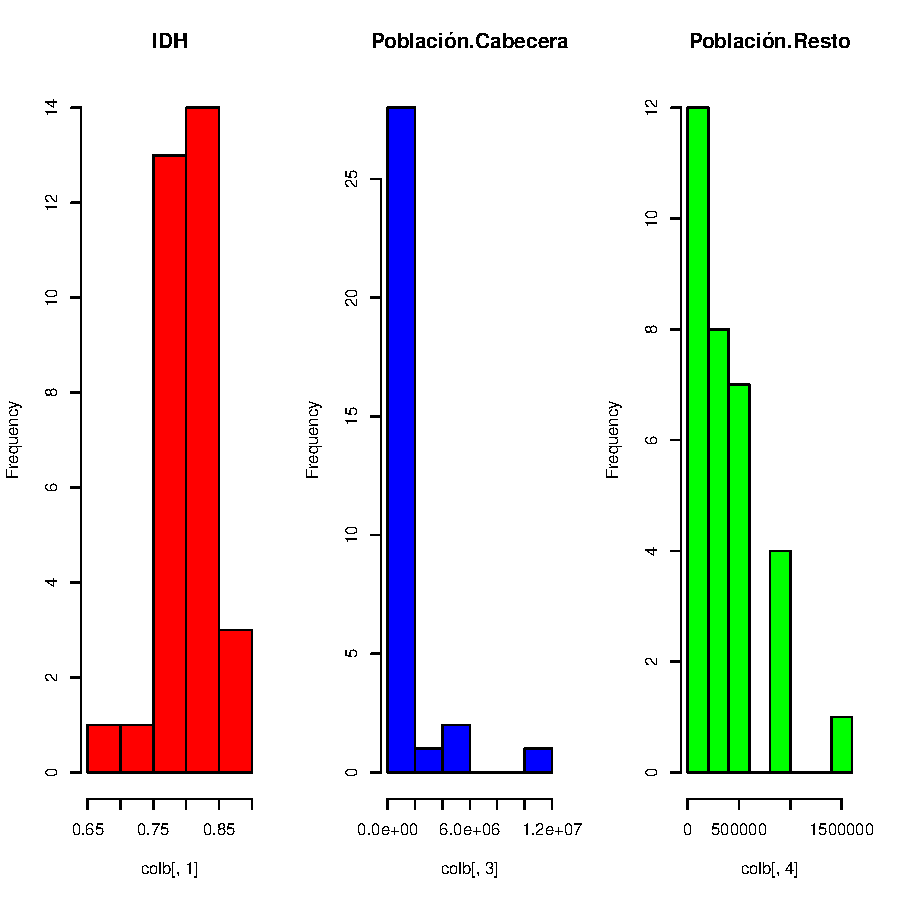
\includegraphics{Proyecto_Final-barplots}
%\end{adjustbox}
\caption{Histogramas}
\label{hist1}
\end{figure}

En cumplimiento de los objetivos misionales del DANE y para que la opinión pública esté informada de la realidad del país, la nueva versión del Atlas busca contribuir a este propósito a través de un lenguaje visual y de la descripción general de tendencias sociodemográficas a lo largo de la geografía del país.

El desarrollo de la nueva obra se emprendió a partir de los resultados del Censo General 2005 y se complementó con fuentes alternas, como registros administrativos y encuestas especializadas del país adelantadas entre los años 2005 y 2010. En los casos en que la información estuvo disponible, se hicieron análisis comparativos con los resultados del Censo de 1993 mostrada en la figura \ref{hist2}.
Además de darle continuidad a la publicación anterior, esta nueva versión del Atlas mantiene la estructura temática, la expresión cartográfica y la organización del contenido de la obra precedente. No obstante, varios de los temas y mapas han sido reconceptualizados o integrados en otros para efectos de una mejor comprensión, utilizando para ello las ventajas de las tecnologías de sistemas de información geográfica.
\clearpage

\begin{figure}[h]
\centering
%\begin{adjustbox}{width=7cm,height=7cm,clip,trim=1.5cm 0.5cm 0cm 1.5cm}
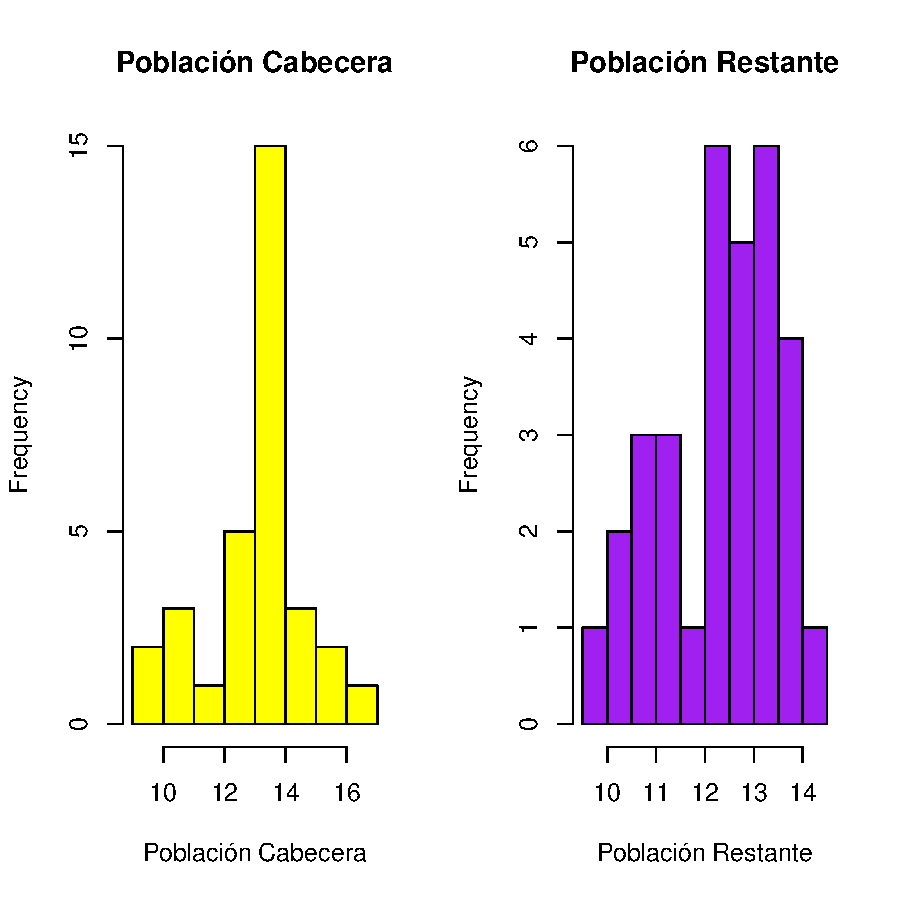
\includegraphics{Proyecto_Final-histnorm}
%\end{adjustbox}
\caption{Histogramas Normalizados}
\label{hist2}
\end{figure}

\section{Exploración Bivariada}

En este trabajo estamos interesados en el impacto de los otros indices en el nivel de Democracia. Veamos las relaciones bivariadas que tiene estas variable con todas las demás:

% Table created by stargazer v.5.2.2 by Marek Hlavac, Harvard University. E-mail: hlavac at fas.harvard.edu
% Date and time: sáb., jun. 30, 2018 - 3:06:45 p. m.
\begin{table}[!htbp] \centering 
  \caption{Correlación de Democracia con las demás variables} 
  \label{corrDem} 
\begin{tabular}{@{\extracolsep{5pt}} cc} 
\\[-1.8ex]\hline 
\hline \\[-1.8ex] 
cabeLog & restoLog \\ 
\hline \\[-1.8ex] 
$0.487$ & $0.177$ \\ 
\hline \\[-1.8ex] 
\end{tabular} 
\end{table} El Departamento Administrativo Nacional de Estadística es un ente estatal que cumple con dos funciones: La primera de carácter técnico- científico que es su razón de ser, pues genera las estadísticas oficiales sobre temas económicos y sociales. Veamos la correlación entre las variables independientes:

% Table created by stargazer v.5.2.2 by Marek Hlavac, Harvard University. E-mail: hlavac at fas.harvard.edu
% Date and time: sáb., jun. 30, 2018 - 3:06:45 p. m.
\begin{table}[!htbp] \centering 
  \caption{Correlación entre variables independientes} 
  \label{corrTableX} 
\begin{tabular}{@{\extracolsep{5pt}} ccc} 
\\[-1.8ex]\hline 
\hline \\[-1.8ex] 
 & cabeLog & restoLog \\ 
\hline \\[-1.8ex] 
cabeLog & 1 &  \\ 
restoLog & 0.84 & 1 \\ 
\hline \\[-1.8ex] 
\end{tabular} 
\end{table} 
Así es como, para mantener una vigilancia sobre el equilibrio o desequilibrio entre los dos factores, se construye un indicador como el Indice de Precios al Consumidor - IPC, que permite monitorear la evolución de los precios de los bienes y servicios que consumen los hogares del país, y guardar registro de ese crecimiento a través del tiempo, a partir de períodos base (mes) del mismo.

%Lo visto en la Tabla \ref{corrTableX} se refuerza claramente en la Figura \ref{corrPlotX}.
\begin{figure}[h]
\centering
\begin{adjustbox}{width=10cm,height=7cm}
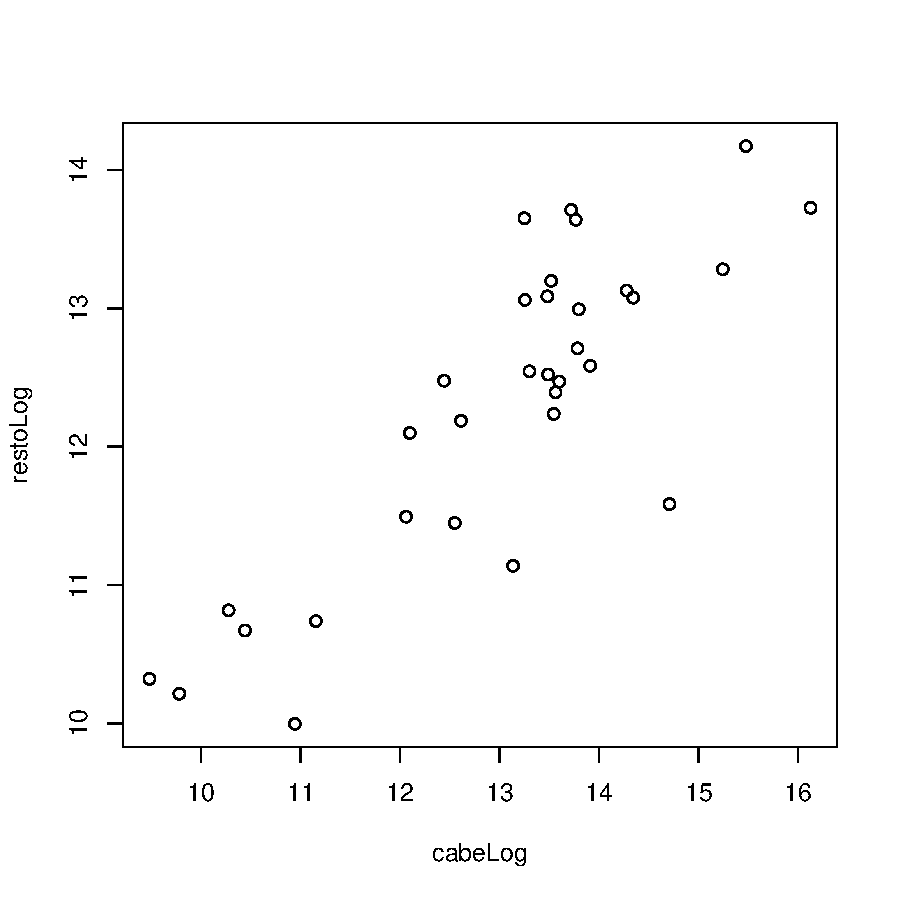
\includegraphics{Proyecto_Final-corrPlotX}
\end{adjustbox}
\caption{correlación entre predictores}
\label{corrPlotX}
\end{figure}

\section{Modelos de Regresión}

Un cambio importante a destacar del nuevo Atlas es que dada la amplia información derivada del censo y de las investigaciones adoptadas, el DANE decidió presentar esta publicación en tres volúmenes \cite{gutierrez_cesar_nodate-1}. El primero de ellos está orientado a los aspectos demográficos y de población; el segundo presenta un panorama general de las condiciones sociales;\cite{panesso-hernandez_localizacion_nodate,} y el tercero presenta información sobre las características y evolución reciente de los principales indicadores económicos con base tanto en la información del Censo General 2005 como de investigaciones que adelanta el DANE regularmente presentadas en la pagina \ref{regresiones} de la página \pageref{regresiones}.



% Table created by stargazer v.5.2.2 by Marek Hlavac, Harvard University. E-mail: hlavac at fas.harvard.edu
% Date and time: sáb., jun. 30, 2018 - 3:06:45 p. m.
\begin{table}[!htbp] \centering 
  \caption{Modelos de Regresión} 
  \label{regresiones} 
\begin{tabular}{@{\extracolsep{5pt}}lcc} 
\\[-1.8ex]\hline 
\hline \\[-1.8ex] 
 & \multicolumn{2}{c}{\textit{Dependent variable:}} \\ 
\cline{2-3} 
\\[-1.8ex] & \multicolumn{2}{c}{IDH} \\ 
\\[-1.8ex] & (1) & (2)\\ 
\hline \\[-1.8ex] 
 cabeLog & 0.013$^{***}$ & 0.031$^{***}$ \\ 
  & (0.004) & (0.007) \\ 
  & & \\ 
 restoLog &  & $-$0.030$^{***}$ \\ 
  &  & (0.010) \\ 
  & & \\ 
 Constant & 0.634$^{***}$ & 0.766$^{***}$ \\ 
  & (0.055) & (0.065) \\ 
  & & \\ 
\hline \\[-1.8ex] 
Observations & 32 & 32 \\ 
R$^{2}$ & 0.238 & 0.425 \\ 
Adjusted R$^{2}$ & 0.212 & 0.385 \\ 
Residual Std. Error & 0.037 (df = 30) & 0.033 (df = 29) \\ 
F Statistic & 9.347$^{***}$ (df = 1; 30) & 10.706$^{***}$ (df = 2; 29) \\ 
\hline 
\hline \\[-1.8ex] 
\textit{Note:}  & \multicolumn{2}{r}{$^{*}$p$<$0.1; $^{**}$p$<$0.05; $^{***}$p$<$0.01} \\ 
\end{tabular} 
\end{table} 
%Como se vió en la Tabla \ref{regresiones}, cuando está presente el \emph{indice de libertad mundial}, el \emph{??ndice de libertad de prensa} pierde significancia.


\section{Exploración Espacial}

Universia Colombia entrevistó a tres profesionales de la Estadística para conocer las motivaciones que los condujeron a estudiar este programa inusual.

El Coordinador del programa de Estadística de la Universidad el Bosque, Ricardo Alberto Borda, contó que "siempre tuve curiosidad e inquietudes sobre la matemática, el cálculo que vi en el colegio y me preguntaba para qué podían servir en la vida real", pero que su elección no solo se basó en su gusto por los números, sino en la posibilidad de ayudar a las personas y líderes en cargos públicos y privados a “tomar a tomar mejores decisiones en diferentes campos laborales”. Estas propuestas en \cite{gower_general_1971}, y para los enlazamientos usaremos la técnica de {\bf medoides} según \cite{macqueen_methods_nodate}. Los tres conglomerados se muestran en la Figura \ref{clustmap}.

\clearpage

El Analista de Datos, Oscar Ayala, declaró que su inclinación por la estadística se debió a la maleabilidad de un campo que parte de los números para ir más allá: “Es mucho más que matemática, es una ciencia muy interesante en donde tienes herramientas matemáticas para poder predecir situaciones”.





\begin{figure}[h]
\centering
%\begin{adjustbox}
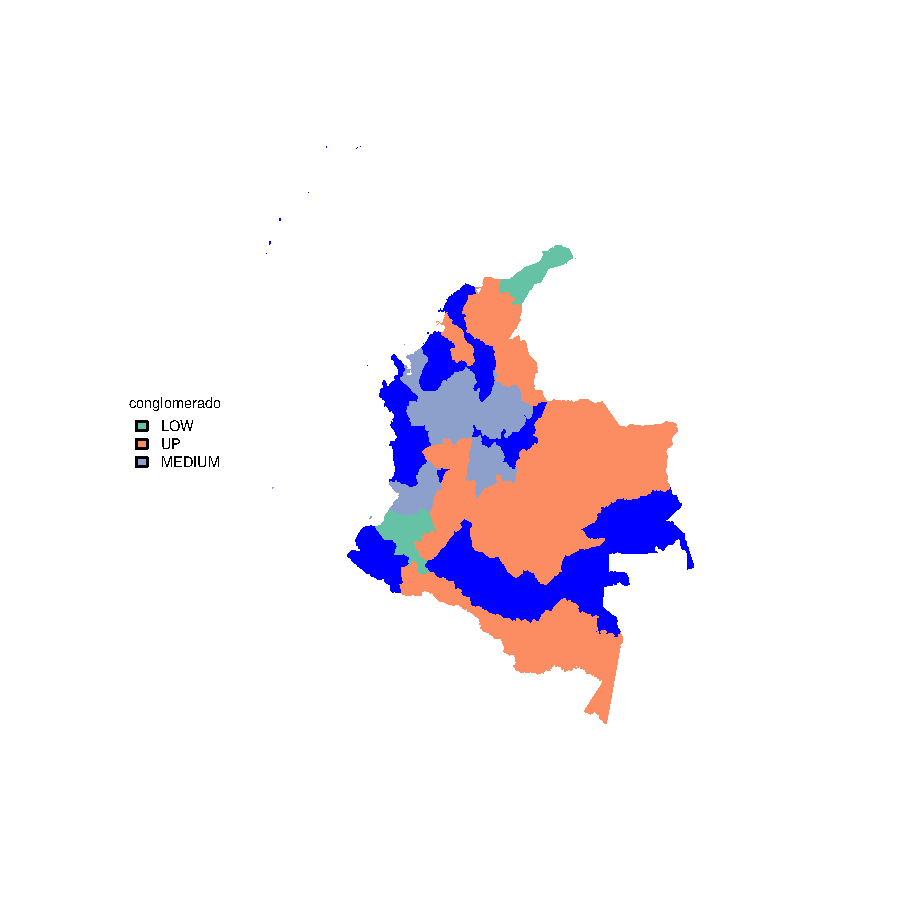
\includegraphics{Proyecto_Final-plotMap1}
%\end{adjustbox}
\caption{Paises conglomerados segun sus indicadores sociopolticos}\label{clustmap}
\end{figure}



%apalike apa
\bibliographystyle{abbrv}
\renewcommand{\refname}{Bibliografia}
\bibliography{Colombia}


\end{document}
